\documentclass{letter}
\usepackage{enumitem}
\usepackage{mathtools}
\usepackage{fancyhdr}
\usepackage{xcolor}
\usepackage{mdframed}
\usepackage{bm}
\usepackage[letterpaper,portrait,left=2cm,right=2cm,top=3.5cm,bottom=2cm]{geometry}
\pagestyle{fancy}

\fancyhf{}
\rhead{Robert Wagner\\June 27, 2016}
\lhead{Math 2101\\Assignment 5}
\newcounter{question}
\setcounter{question}{0}
\usepackage{amsmath,amsthm}
\usepackage{amssymb}
\usepackage{tikz}
\usetikzlibrary{arrows}


% magnitude bars
\newcommand{\norm}[1]{\lvert #1 \rvert}

% explicit vector
\newcommand{\Ve}[1]{\langle #1 \rangle}

% named vector
\newcommand{\Vn}[1]{\vec{#1}}

% a line with an arrow above
\newcommand{\Line}[1]{\overrightarrow{#1}}

% equals with question mark above
\newcommand{\?}{\stackrel{?}{=}}

% formatting for questions
\newcommand\Que[1]{%
   \leavevmode\noindent
   #1
}

% formatting for answers
\newcommand\Ans[2][]{%
   \leavevmode\noindent
   {
       \begin{mdframed}[backgroundcolor=blue!10]
       #2
       \end{mdframed}
   }
}

% this is like align but squashed     
\newenvironment{salign}
 {\par$\!\aligned}
 {\endaligned$\par}

% a matrix, parameter is column count
\newenvironment{Mat}[1]{%
  \left[\begin{array}{*{#1}{r}}
}{%
  \end{array}\right]
}
% a matrix, parameter is column count centered
\newenvironment{Cmat}[1]{%
  \left[\begin{array}{*{#1}{c}}
}{%
  \end{array}\right]
}

% an augmented matrix, with one augmented column
\newenvironment{Amat}[1]{%
  \left[\begin{array}{@{}*{#1}{r}|r@{}}
}{%
  \end{array}\right]
}
% an augmented matrix with n columns and n augmented columns
\newenvironment{Amat2}[1]{%
  \left[\begin{array}{@{~}*{#1}{r}| @{~~}*{#1}{r}}
}{%
  \end{array}\right]
}
% an augmented matrix with n columns and m augmented columns
\newenvironment{Amat3}[2]{%
  \left[\begin{array}{@{~}*{#1}{r}| @{~~}*{#2}{r}}
}{%
  \end{array}\right]
}


\begin{document}


\begin{enumerate}
    \item For each of the following, find a basis for Row(A), Col(A), and Null(A); also identify the dimension of each.  If the vectors are not independent, express the dependent vector(s) as linear combinations of the others.
    \begin{enumerate}
    \item $A= \begin{Mat}{3} 2 & 3 & 1 \\ 1 & 2 & 5 \\ 0 & 3 & 1 \end{Mat} $
    \Ans{
       First, we find rref($A$) to find bases for Col($A$) and Null($A$)
       \begin{align*}
           &\begin{Mat}{3} 2 & 3 & 1 \\ 1 & 2 & 5 \\ 0 & 3 & 1 \end{Mat} 
           \to
           \begin{Mat}{3} 1 & 1 & -4 \\ 1 & 2 & 5 \\ 0 & 3 & 1 \end{Mat}
           \to
           \begin{Mat}{3} 1 & 1 & -4 \\ 0 & 1 & 9 \\ 0 & 3 & 1 \end{Mat}
           \to
           \begin{Mat}{3} 1 & 1 & -4 \\ 0 & 1 & 9 \\ 0 & 0 & -26 \end{Mat}
           \to
           \cdots
           \to
           \begin{Mat}{3} 1 & 0 & 0 \\ 0 & 1 & 0 \\ 0 & 0 & 1 \end{Mat}
           \shortintertext{Since each column in rref($A$) has a pivot we can see a basis for Col($A$) is $\{\Ve{2,1,0}^T,\Ve{3,2,3}^T,\Ve{1,5,1}^T\}$\ with dimension 3, and the basis for Null($A$) is $\{\Ve{0,0,0}^T\}$\ with dimension 0.  All columns are independent.}
           &~\\
           \shortintertext{Now we find rref($A^T$) to find a basis for Row($A$)}
           &\begin{Mat}{3} 2 & 1 & 0 \\ 3 & 2 & 3 \\ 1 & 5 & 1 \end{Mat}
           \to
           \begin{Mat}{3} 1 & -4 & -1 \\ 0 & -13 & 0 \\ 1 & 5 & 1 \end{Mat}
           \to
           \begin{Mat}{3} 1 & -4 & -1 \\ 0 & 1 & 0 \\ 0 & 9 & 2 \end{Mat}
           \to
           \begin{Mat}{3} 1 & 0 & -1 \\ 0 & 1 & 0 \\ 0 & 0 & 2 \end{Mat}
           \to
           \begin{Mat}{3} 1 & 0 & 0 \\ 0 & 1 & 0 \\ 0 & 0 & 1 \end{Mat}
           \shortintertext{So we can see a basis for Row($A$) is $\{\Ve{2,3,1},\Ve{1,2,5},\Ve{0,3,1}\}$\ with dimension 3.}
       \end{align*}
    }
    \item $A= \begin{Mat}{4} 1 & 3 & 1 & 2 \\ 2 & 3 & 1 & 0 \\ 4 & -1 & -2 & 1 \end{Mat}$
    \Ans{
        First, we find rref($A$) to find bases for Col($A$) and Null($A$):
        \begin{align*}
            &\begin{Mat}{4} 1 & 3 & 1 & 2 \\ 2 & 3 & 1 & 0 \\ 4 & -1 & -2 & 1 \end{Mat}
            \to
            \begin{Mat}{4} 1 & 3 & 1 & 2 \\ 0 & -3 & -1 & -4 \\ 0 & -13 & -6 & -7 \end{Mat}
            \to
            \begin{Mat}{4} 1 & 3 & 1 & 2 \\ 0 & 39 & 13 & 52 \\ 0 & -39 & -18 & -21 \end{Mat}
            \to
            \begin{Mat}{4} 1 & 3 & 1 & 2 \\ 0 & 3 & 1 & 4 \\ 0 & 0 & -5 & 31 \end{Mat}
            \to\\
            &\begin{Mat}{4} 1 & 0 & 0 & -2 \\ 0 & 3 & 1 & 4 \\ 0 & 0 & -5 & 31 \end{Mat}
            \to
            \begin{Mat}{4} 1 & 0 & 0 & -2 \\ 0 & 15 & 5 & 20 \\ 0 & 0 & -5 & 31 \end{Mat}
            \to
            \begin{Mat}{4} 1 & 0 & 0 & -2 \\ 0 & 15 & 0 & 51 \\ 0 & 0 & -5 & 31 \end{Mat}
            \to
            \begin{Mat}{4} 1 & 0 & 0 & -2 \\ 0 & 1 & 0 & 51/15 \\ 0 & 0 & 1 &-31/5 \end{Mat}
            \shortintertext{Since columns 1, 2, 3 have pivots we can see a basis for Col($A$) is $\{\Ve{1,2,4}^T,\Ve{3,3,-1}^T,\Ve{1,1,-2}^T\}$\ with dimension 3.}
            \shortintertext{and a basis for Null($A$) is $\{\Ve{30,-51,93,15}^T\}$\ with dimension 1.}
            \shortintertext{column 4 is dependent on the others, and can be expressed as $-2\Ve{1,2,4}^T+\frac{51}{15}\Ve{3,3,-1}^T-\frac{31}{5}\Ve{1,1,-2}^T$}
            &~\\
            \shortintertext{Now, we find rref($A^T$) to find basis for Row(A):}
            &\begin{Mat}{3} 1 & 2 & 4 \\ 3 & 3 & -1 \\ 1 & 1 & -2 \\ 2 & 0 & 1 \end{Mat}
            \to
            \begin{Mat}{3} 1 & 2 & 4 \\ 0 & -3 & -13 \\ 0 & -1 & -6 \\ 0 & -4 & -7 \end{Mat}
            \to
            \begin{Mat}{3} 1 & 2 & 4 \\ 0 & 1 & -6 \\ 0 & -1 & -6 \\ 0 & -4 & -7 \end{Mat}
            \to
            \begin{Mat}{3} 1 & 2 & 4 \\ 0 & 1 & -6 \\ 0 & 0 & -12 \\ 0 & 0 & -31 \end{Mat}
            \to\cdots\to
            \begin{Mat}{3} 1 & 0 & 0 \\ 0 & 1 & 0 \\ 0 & 0 & 1 \\ 0 & 0 & 0 \end{Mat}
            \shortintertext{Since rows 1, 2, 3 have pivots, we can see a basis for Row($A$) is $\{\Ve{1,3,1,2},\Ve{2,3,1,0},\Ve{4,-1,-2,1}\}$\ with dimension 3.} 
        \end{align*}
    }    
    \newpage
    \item $A= \begin{Mat}{3} 3 & 1 & 4 \\1 & 5 & 9 \\ 2 & -4 & -5 \end{Mat} $ 
    \Ans{
    First, we find rref($A$) to find bases for Col($A$) and Null($A$):
        \begin{align*}
            &\begin{Mat}{3} 3 & 1 & 4 \\ 1 & 5 & 9 \\ 2 & -4 & -5 \end{Mat}
            \to
            \begin{Mat}{3} 1 & 5 & 9 \\ 1 & 5 & 9 \\ 2 & -4 & -5 \end{Mat}
            \to
            \begin{Mat}{3} 1 & 5 & 9 \\ 0 & -14 & -23 \\ 0 & 0 & 0 \end{Mat}
            \to
            \begin{Mat}{3} 1 & 5 & 9 \\ 0 & 1 & 23/14 \\ 0 & 0 & 0 \end{Mat}
            \to
            \begin{Mat}{3} 1 & 0 & 11/14 \\ 0 & 1 & 23/14 \\ 0 & 0 & 0 \end{Mat}
            \shortintertext{Since columns 1, 2 have pivots we can see a basis for Col($A$) is $\{\Ve{3,1,2}^T,\Ve{1,5,-4}^T\}$\ with dimension 2.}
            \shortintertext{and a basis for Null($A$) is $\{\Ve{-11,-23,14}^T\}$\ with dimension 1.}
            \shortintertext{column 3 is dependent on the others, and can be expressed as $\frac{11}{14}\Ve{3,1,2}^T+\frac{23}{14}\Ve{1,5,-4}^T$}
        \end{align*}
    }    
    \end{enumerate}
    ~\\     
    \item 
        Let $\mathbb{V}=\{\Vn{v}_1,\Vn{v}_2\}$ be a basis for a 2-dimensional vector space, and let
        \begin{align*}
            \Vn{w}_1 &= a_{11}\Vn{v}_1 + a_{12}\Vn{v}_2 \\
            \Vn{w}_2 &= a_{21}\Vn{v}_1 + a_{22}\Vn{v}_2
        \end{align*} 
        where all $a_{ij} \in \mathbb{R}$.
    \begin{enumerate}[label=(\alph*)]
    \item \Que{
        Under what conditions will $\mathbb{W}=\{\Vn{w}_1,\Vn{w}_2\}$\ be the basis of a 2-dimensional vector space?        
    }
    \Ans{
       $\Vn{w}_1$\ and $\Vn{w}_2$\ will be a basis if they do not point in the same direction.  Since $\Vn{v}_1$\ and $\Vn{v}_2$\ form a basis, we know we can meet this condition by making sure the ratio between components of $\Vn{v}_i$\ are not the same in $\Vn{w}_i$.
       \begin{align*}
           \frac{a_{11}}{a_{21}} &\not = \frac{a_{12}}{a_{22}}
           \shortintertext{since we do not know that $a_{21}\not = 0, a_{22}\not = 0$\ it is better to say}
           a_{11}a_{22} &\not = a_{12}a_{21} \\
           a_{11}a_{22}-a_{12}a_{21} &\not = 0
       \end{align*}
       And we see that this is analogous to the conditions for matrix invertibility in assignment 4 question 2.  
       Thus we can deduce that if 
       \[A=\begin{Mat}{2} a_{11} & a_{12} \\ a_{21} & a_{22} \end{Mat} \] 
       is an invertible matrix corresponding to a change of basis transformation performed on a set of basis vectors then the outcome is a set of basis vectors.  
    }
    \newpage
    \item \Que{
        Prove or disprove: If $\mathbb{W}$\ is the basis for a 2-dimensional vector space, it will be the same as the vector space spanned by $\mathbb{V}$.    
    }
    \Ans{
     Suppose $\mathbb{W}$\ is a basis for a 2d vector space.  Let $\Vn{x} \in Span(\mathbb{W})$\ such that $\Vn{x}=x_1\Vn{w}_1+x_2\Vn{w}_2$ for some $x_1,x_2 \in \mathbb{R}$\ not both zero.
     \begin{align*}
         \Vn{w}&=x_1\Vn{w}_1+x_2\Vn{w}_2\\
               &=x_1(a_{11}\Vn{v}_1+a_{12}\Vn{v}_2)+x_2(a_{21}\Vn{v}_1+a_{22}\Vn{v}_2)\\
               &=(x_1a_{11}+x_2a_{21})\Vn{v}_1+(x_1a_{12}+x_2a_{22})\Vn{v}_2
     \end{align*}
     thus $\Vn{x} \in Span(\mathbb{V})$\ and $Span(\mathbb{W})\subseteq Span(\mathbb{V})$.\\
     Let $\Vn{y}\in Span(\mathbb{V})$\ such that $\Vn{y}=y_1\Vn{v}_1+y_2\Vn{v}_2$\ for some $y_1,y_2 \in \mathbb{R}$\ not both zero.  
     \begin{align*}
         \Vn{y}&=y_1\Vn{v}_1+y_2\Vn{y}_2
         \intertext{since we know $a_{11}a_{22}-a_{12}a_{21}\not = 0$\ we can substitute $y_1=x^\prime, y_2=y^\prime$\ found in part c below:}
         \Vn{v}&=x^\prime\Vn{w}_1 + y^\prime\Vn{w}_2\\ 
               &= \frac{y_1\cdot a_{22} - y_2\cdot a_{21}}{a_{11}a_{22}-a_{12}a_{21}}\Vn{w}_1 +
                  \frac{y_2\cdot a_{11}-y_1\cdot a_{12}}{a_{11}a_{22}-a_{12}a_{21}}\Vn{w}_2
     \end{align*}
     By the answer to 2(c) below.  Thus $\Vn{y}\in Span(\mathbb{W}), Span(\mathbb{V})\subseteq Span(\mathbb{W})$, and subsequently\\
     $Span(\mathbb{V})=Span(\mathbb{W})$.
    }
    ~\\
    %\newpage
    \item \Que{
        Suppose $\Vn{x}=a\Vn{v}_1+b\Vn{v}_2$.  Find $a^\prime, b^\prime$\ so that $\Vn{x}=a^\prime\Vn{w}_1 + b^\prime\Vn{w}_2$.
    }
    \Ans{
      
      Let $A=\begin{Mat}{2} a_{11} & a_{12} \\ a_{21} & a_{22} \end{Mat}$.  
      By the definition above $A\begin{Mat}{1} \Vn{v}_1 \\ \Vn{v}_2 \end{Mat} = \begin{Mat}{1} \Vn{w}_1 \\ \Vn{w}_2 \end{Mat}$.  Multiply both sides by $A^{-1}$:
      \begin{align*}
       A^{-1}A\begin{Mat}{1} \Vn{v}_1 \\ \Vn{v}_2 \end{Mat}
       &= 
       A^{-1}\begin{Mat}{1} \Vn{w}_1 \\ \Vn{w}_2 \end{Mat}
       = \frac{1}{a_{11}a_{22}-a_{12}a_{21}}\begin{Mat}{2} a_{22} & -a_{12} \\ -a_{21} & a_{11} \end{Mat}\begin{Mat}{1} \Vn{w}_1 \\ \Vn{w}_2 \end{Mat}
       \shortintertext{thus}
       \Vn{x} &= \begin{Mat}{2}a & b \end{Mat} \begin{Mat}{1} \Vn{v}_1 \\ \Vn{v}_2 \end{Mat}
       = \begin{Mat}{2}a & b \end{Mat} \frac{1}{a_{11}a_{22}-a_{12}a_{21}}\begin{Mat}{2} a_{22} & -a_{12} \\ -a_{21} & a_{11} \end{Mat}\begin{Mat}{1} \Vn{w}_1 \\ \Vn{w}_2 \end{Mat}\\
       \begin{Mat}{2} a^\prime & b^\prime \end{Mat} 
       &= \frac{1}{a_{11}a_{22}-a_{12}a_{21}}\begin{Mat}{2}a & b \end{Mat} \begin{Mat}{2} a_{22} & -a_{12} \\ -a_{21} & a_{11} \end{Mat}
       =  \underline{\begin{Mat}{2} \frac{a\cdot a_{22} - b\cdot a_{21}}{a_{11}a_{22}-a_{12}a_{21}} & \frac{b\cdot a_{11}-a\cdot a_{12}}{a_{11}a_{22}-a_{12}a_{21}} \end{Mat}}
      \end{align*}
    }
    \end{enumerate}
    %~\\
    \newpage
    \item
        The following will prove a useful theorem about independence, and motivate why we care about it.  Suppose
        $\mathbb{V} = \{\Vn{v}_1, \Vn{v}_2, \cdots,\Vn{v}_n\}$\ is a set of $n$\ vectors, none of which is the zero vector.  Let $x=\sum^n_{i=1} a_i\Vn{v}_i$.  
    \begin{enumerate}[label=(\alph*)]  
      \item \Que{
      Suppose $x=(a_1,a_2,\cdots,a_n)$\ and also $x=(b_1,b_2,\cdots,b_n)$, 
      where $a_i\not = b_i$\ for at least one $i$.  Show that this means $\Vn{0}=\sum^n_{i=1}c_i\Vn{v}_i$, 
      where at least one $c_i$\ is non-zero.
      }
      \Ans{
          Let $j\in \{1,2,\cdots,n\}$\ such that $a_j\not = b_j$.  It follows that $b_j-a_j\not = 0$.  Since $x=\sum^n_{i=1}a_i\Vn{v}_i = \sum^n_{i=1}b_i\Vn{v}_i$
          \begin{align*}
              x&=\begin{Mat}{4}          &          &        &         \\
                             \Vn{v}_1 & \Vn{v}_2 & \cdots & \Vn{v}_n \\ 
                                      &          &        &   \end{Mat}
              \begin{Mat}{1} a_1 \\ a_2 \\ \vdots \\ a_n \end{Mat} 
              = 
              \begin{Mat}{4}          &          &        &         \\
                             \Vn{v}_1 & \Vn{v}_2 & \cdots & \Vn{v}_n \\ 
                                      &          &        &   \end{Mat}
              \begin{Mat}{1} b_1 \\ b_2 \\ \vdots \\ b_n \end{Mat} \\
              \Vn{0} &=
              \begin{Mat}{4}          &          &        &         \\
                             \Vn{v}_1 & \Vn{v}_2 & \cdots & \Vn{v}_n \\ 
                                      &          &        &   \end{Mat}
              \begin{Mat}{1} b_1 \\ b_2 \\ \vdots \\ b_n \end{Mat}
              -\begin{Mat}{4}          &          &        &         \\
                             \Vn{v}_1 & \Vn{v}_2 & \cdots & \Vn{v}_n \\ 
                                      &          &        &   \end{Mat}
              \begin{Mat}{1} a_1 \\ a_2 \\ \vdots \\ a_n \end{Mat} \\
              \Vn{0} &= \begin{Cmat}{1} v_1^1b_1+v_1^2b_2+\cdots+v_1^jb_j+\cdots+v_1^nb_n \\
                                        v_2^1b_1+v_2^2b_2+\cdots+v_2^jb_j+\cdots+v_2^nb_n \\
                                        \vdots \\
                                        v_n^1b_1+v_n^2b_2.\cdots+v_j^nb_j+\cdots+v_n^nb_n \end{Cmat}
              -
                        \begin{Cmat}{1} v_1^1a_1+v_1^2a_2+\cdots+v_1^ja_j+\cdots+v_1^na_n \\
                                        v_2^1a_1+v_2^2a_2+\cdots+v_2^ja_j+\cdots+v_2^na_n \\
                                        \vdots \\
                                        v_n^1a_1+v_n^2a_2.\cdots+v_j^na_j+\cdots+v_n^na_n \end{Cmat}  \\       
              \Vn{0} &= \begin{Cmat}{1} (b_1-a_1)v_1^1+(b_2-a_2)v_1^2+\cdots+(b_j-a_j)v_1^j+\cdots+(b_n-a_n)v_1^n \\
                                        (b_1-a_1)v_2^1+(b_2-a_2)v_2^2+\cdots+(b_j-a_j)v_2^j+\cdots+(b_n-a_n)v_2^n \\
                                        \vdots \\
                                        (b_1-a_1)v_n^1+(b_2-a_2)v_n^2+\cdots+(b_j-a_j)v_n^j+\cdots+(b_n-a_n)v_n^n \end{Cmat} \\
              \Vn{0} &=\begin{Mat}{6}          &          &        &          &        & \\
                                      \Vn{v}_1 & \Vn{v}_2 & \cdots & \Vn{v}_j & \cdots & \Vn{v}_n \\ 
                                               &          &        &          &        & \end{Mat}
              \begin{Mat}{1} b_1-a_1 \\ b_2-a_2 \\ \vdots \\ b_j-a_j \\ \vdots \\ b_n-a_n \end{Mat}   
              = \sum^n_{i=1} (b_i-a_i)\Vn{v}_i                 
          \end{align*}
          Let $\Vn{c}=\Vn{b}-\Vn{a}$.  Since $b_j-a_j \not = 0$\ it follows that there is at least one $c_i$\ that is non-zero.
      }      
      %\newpage
      ~\\
      \item \Que {
      Suppose $x=(a_1,a_2,\cdots,a_n)$\ and also $x=(b_1,b_2,\cdots,b_n)$\ as above.  Show that if $y=(p_1,p_2,\cdots,p_n)$, then $y=(q_1,q_2,\cdots,q_n)$\ where $p_i\not = q_i$\ for at least one $i$.   
      }
      \Ans{
      Let $j\in \{1,2,\cdots,n\}$\ such that $a_j\not = b_j$.  It follows that $a_j-b_j\not = 0$.  Suppose $y=(p_1,p_2,\cdots,p_n)$.
      \begin{align*}
          x+y&=(a_1\Vn{v}_1 + \cdots + a_j\Vn{v}_j+\cdots+a_n\Vn{v}_n) + (p_1\Vn{v}_1 + \cdots + p_j\Vn{v}_j+\cdots+p_n\Vn{v}_n)\\
          x-x+y &=(a_1\Vn{v}_1 + \cdots + a_j\Vn{v}_j+\cdots+a_n\Vn{v}_n) - (b_1\Vn{v}_1 + \cdots + b_j\Vn{v}_j+\cdots+b_n\Vn{v}_n)\\
                &+ (p_1\Vn{v}_1 + \cdots + p_j\Vn{v}_j+\cdots+p_n\Vn{v}_n)\\
          y &= (a_1-b_1+p_1)\Vn{v}_1+\cdots+(a_j-b_j+p_j)\Vn{v}_j+\cdots+(a_n-b_n+p_n)\Vn{v}_n
       \shortintertext{Let $q_i = a_i-b_i+p_1$\ for all $i\in \{1\cdots n\}$.}
          y &= q_1\Vn{v}_1 + \cdots + q_j\Vn{v}_j + \cdots + q_n\Vn{v}_n      
      \end{align*}
       Since $a_j-b_j \not = 0$\ it follows that $q_j\not = p_j$\ thus $y=(q_1,q_2,\cdots,q_n)$\ where $p_i\not = q_i$\ for at least one $i$.
      }
      \item \Que {
      Suppose the zero vector can be expressed as a non-trivial linear combination of the vectors in $\mathbb{V}$.  	
      Show that this means that the vectors of $\mathbb{V}$\ are not independent.
      }
      \Ans{
          Suppose $\Vn{0}$\ is a non-trivial linear combination of vectors in $\mathbb{V}$\ with at least one $c_i\not =0$.  Let $j\in\{1,2,\cdots,n\}$\ such that $c_j\not = 0$.
          \begin{align*}
              \Vn{0}       &= c_1\Vn{v}_1+\cdots+c_j\Vn{v}_j+\cdots+c_n\Vn{v}_n\\
              -c_j\Vn{v}_j &=c_1\Vn{v}_1+\cdots+c_{j-1}\Vn{v}_{j-1}+c_{j+1}\Vn{v}_{j+1}+\cdots+c_n\Vn{v}_n\\
              \Vn{v}_j     &=\frac{c_1}{-c_j}\Vn{v}_1 + \cdots + \frac{c_{j-1}}{-c_j}\Vn{v}_{j-1}+
                             \frac{c_{j+1}}{-c_j}\Vn{v}_{j+1}+\cdots+\frac{c_n}{-c_j}\Vn{v}_n
          \end{align*}   
          Thus we have shown that $\Vn{v}_j$\ is a linear combination of the other vectors, therefore the vectors of $\mathbb{V}$\ are not independent.
      }
      \item \Que {
      Suppose the vectors of $\mathbb{V}$\ are independent.  Show this implies $\Vn{0}=\sum^n_{i=1}a_i\Vn{v}_i$ has a unique solution.  
      }
      \Ans{
      Let $\Vn{a}=\Ve{a_1,a_2,\cdots,a_n}$\ and $\Vn{b}=\Ve{b_1,b_2,\cdots,b_n}$\ such that $\sum^n_{i=1}a_i\Vn{v}_i = \sum^n_{i=1}b_i\Vn{v}_i$.  Let $j \in \{1\cdots n\}$. 
      \begin{align*}
          a_1\Vn{v}_1+\cdots+a_n\Vn{v}_n &= b_1\Vn{v}_1+b_2\Vn{v}_2+\cdots+b_n\Vn{v}_n\\
          \Vn{0} &= b_1\Vn{v}_1+b_2\Vn{v}_2+\cdots+b_n\Vn{v}_n - a_1\Vn{v}_1+a_2\Vn{v}_2+\cdots+a_n\Vn{v}_n \\
                 &= (b_1-a_1)\Vn{v}_1 + (b_2-a_2)\Vn{v}_2 + \cdots + (b_j-a_j)\Vn{v}_j+\cdots+(b_n-a_n)\Vn{v}_n 
        \shortintertext{subtracting the scaled multiple of $\Vn{v}_j$\ from both sides results in}
          (a_j-b_j)\Vn{v}_j &= (b_1-a_1)\Vn{v}_1 + \cdots + (b_{j-1}-a_{j-1})\Vn{v}_{j-1}+
                               (b_{j+1}-a_{j+1})\Vn{v}_{j+1}+\cdots+(b_n-a_n)\Vn{v}_n\\
          \Vn{v}_j &= \frac{b_1-a_1}{a_j-b_j}\Vn{v}_1 + \cdots + \frac{b_{j-1}-a_{j-1}}{a_j-b_j}\Vn{v}_{j-1} + 
                               \frac{b_{j+1}-a_{j+1}}{a_j-b_j}\Vn{v}_{j+1}+\cdots+\frac{b_n-a_n}{a_j-b_j}\Vn{v}_n
          \shortintertext{since the vectors of $\mathbb{V}$\ are independent, it cannot be the case that $\Vn{v}_j$\ is a linear combination of the other vectors, therefore $a_k-b_k=0$\ and subsequently $a_k=b_k$\ must be true for all $k \in \{1\cdots n\}$.  Returning to the step}
          \Vn{0}&= (b_1-a_1)\Vn{v}_1 + (b_2-a_2)\Vn{v}_2 + \cdots + (b_j-a_j)\Vn{v}_j+\cdots+(b_n-a_n)\Vn{v}_n \\
                &= \sum^n_{i=1}(b_i-a_i)\Vn{v}_i 
                = \sum^n_{i=1}0\Vn{v}_i 
                = 0\sum^n_{i=1}\Vn{v}_i
      \end{align*}   
      And we have thus shown there is a singular solution $x=\Ve{0,\cdots,0}$\ for $\Vn{0}=\sum^n_{i=1}x_i\Vn{v}_i$.
      }
      %\newpage
      \item \Que{
      Show that if $\Vn{0}=\sum^n_{i=1}a_i\Vn{v}_i$\ has a unique solution, then the vectors of $\mathbb{V}$\ are independent.
      }
      \Ans{
          Suppose that there exists $j\in\{1,\cdots,n\}$\ such that 
          $b_j\Vn{v}_j = b_1\Vn{v}_1 + \cdots + b_{j-1}\Vn{v}_{j-1} + b_{j+1}\Vn{v}_{j+1}+\cdots+b_n\Vn{v}_n$ for some $b_1,\cdots,b_n\in\mathbb{R}$, i.e. the vectors are not independent.    
         \begin{align*}
         b_j\Vn{v}_j &= b_1\Vn{v}_1 + \cdots + b_{j-1}\Vn{v}_{j-1} + b_{j+1}\Vn{v}_{j+1}+\cdots+b_n\Vn{v}_n \\
         \Vn{0} &= b_1\Vn{v}_1 + \cdots + (-b_j)\Vn{v}_j+\cdots+b_n\Vn{v}_n \\
         (-1)\Vn{0} = \Vn{0} &= (-b_1)\Vn{v}_1 + \cdots + b_j\Vn{v}_j+\cdots+(-b_n)\Vn{v}_n
         \end{align*}
         Thus we have found two solutions for $\Vn{0}=\sum^n_{i=1}a_i\Vn{v}_i$:
         \begin{align*}
             a&=\Ve{b_1,\cdots,-b_j,\cdots,b_n}\\
             a^\prime&=\Ve{-b_1,\cdots,b_j,\cdots,-b_n}
         \end{align*}
         Thus if the vectors are not independent then there is not a unique solution to $\Vn{0}=\sum^n_{i=1}a_i\Vn{v}_i$, and by contrapositive if there is a unique solution to $\Vn{0}=\sum^n_{i=1}a_i\Vn{v}_i$\ then the vectors are independent.
      }
    \end{enumerate}
    %~\\
    \item
        A set of vectors $\mathbb{V}$\ is said to be orthogonal if any two vectors are perpendicular.
    \begin{enumerate}[label=(\alph*)]
    \item \Que{
        Let $\mathbb{V}=\{\Vn{v}_1,\Vn{v}_2\}$, and assume these form a basis.  Find a vector $\Vn{v}_{2\perp}$\ that is perpendicular to $\Vn{v}_1$.  
    }
    \Ans{
        
          \begin{minipage}[m]{0.6\textwidth}
            \begin{salign}
             \Vn{v}_{2\perp} &= \Vn{v}_2 - proj_{\Vn{v}_1}\Vn{v_2} \\
                             &= \Vn{v}_2 - (\norm{\Vn{v}_2}\cos\theta) \frac{\Vn{v}_1}{\norm{\Vn{v}_1}}\\
                             &= \Vn{v}_2 - \left(\frac{\norm{\Vn{v}_2}}{\norm{\Vn{v}_1}}\right)
                                           \left(\frac{\Vn{v}_1\cdot\Vn{v}_2}{\norm{\Vn{v}_1}\norm{\Vn{v}_2}}\right)\Vn{v}_1\\
                             &= \Vn{v}_2 - \left(\frac{\Vn{v}_1\cdot\Vn{v}_2}{\norm{\Vn{v}_1} \norm{\Vn{v}_1}}\right)\Vn{v}_1 \\
                             &= \Vn{v}_2 - \frac{\Vn{v}_1\cdot\Vn{v}_2}{\Vn{v}_1\cdot\Vn{v}_1}\Vn{v}_1
            \end{salign}
          \end{minipage}
          \begin{minipage}[m]{0.3\textwidth}
            \centering
            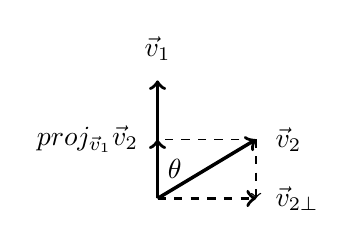
\begin{tikzpicture}[x=1cm,y=1cm]
                \draw[->, line width = 1.25pt](0,0)--(0,1.5);
                \draw[->, line width = 1.25pt](0,0)--(1.25,0.75);
                \draw[->, dashed, line width = 1.25pt](0,0)--(1.25,0);
                \draw[-, dashed, line width = 0.5pt](1.25,0.75)--(0,0.75);
                \draw[->, dashed, line width = 0.5pt](1.25,0.75)--(1.25,0);
                \draw[->, line width=1.25pt](0,0)--(0,0.75);
                \node[label={180:{$proj_{\Vn{v}_1}\Vn{v}_2$}}] at (0,0.75) {};
                \node[label={90:{$\Vn{v}_1$}}] (P) at (0,1.5) {};
                \node[label={0:{$\Vn{v}_2$}}] (P') at (1.25, 0.75) {}; 
                \node[label={0:{$\Vn{v}_{2\perp}$}}] (P'') at (1.25,0) {};    
                \node[label={87.5:{$\theta$}}] (origin) at (0,0) {};     
                %\draw[->] (1,1.5) (P) to [bend left] (P'); 
            \end{tikzpicture}
          \end{minipage}
    }
    \item \Que{
        Show that $\mathbb{V}_\perp = \{\Vn{v}_1,\Vn{v}_{2\perp}\}$\ consists of a set of independent vectors.
    }
    \Ans{ 
        Suppose $\mathbb{V}_\perp$\ is not independent, thus there exists $x_1,x_2 \in\mathbb{R}$\ such that  $\Vn{0}=x_1\Vn{v}_1 + x_2\Vn{v}_{2\perp}$\ and at least one $x_i$\ is non-zero. 
        \begin{align*}
            \Vn{0} &= x_1\Vn{v}_1 + x_2\Vn{v}_{2\perp}\\
            \Vn{0} &= x_1\Vn{v}_1 + x_2\left(\Vn{v}_2 - \frac{\Vn{v}_1\cdot\Vn{v}_2}{\Vn{v}_1\cdot\Vn{v}_1}\Vn{v}_1\right)
                   = \left(x_1-x_2\frac{\Vn{v}_1\cdot\Vn{v}_2}{\Vn{v}_1\cdot\Vn{v}_1}\right)\Vn{v}_1 + x_2\Vn{v}_2
            \shortintertext{since we know that $\Vn{v}_1, \Vn{v}_2$\ form a basis, we know that only the trivial solution to $\Vn{0}=x_1^\prime\Vn{v}_1+x_1^\prime\Vn{v}_2$\ exists, thus $x_1^\prime=0$\ and $x_2^\prime=0$\ and}
            x_2\prime&=x_2=0\\
            x_1\prime&=x_1-x_2\frac{\Vn{v}_1\cdot\Vn{v}_2}{\Vn{v}_1\cdot\Vn{v}_1}=0 \\
            x_1&= x_2\frac{\Vn{v}_1\cdot\Vn{v}_2}{\Vn{v}_1\cdot\Vn{v}_1} + x_1^\prime 
               = 0\frac{\Vn{v}_1\cdot\Vn{v}_2}{\Vn{v}_1\cdot\Vn{v}_1}+0 = 0
        \end{align*}
        And we have reached a contradiction since $x_1=0$\ and $x_2=0$\ contradicts our initial claim that at least one is non-zero.
        Therefore $\mathbb{V}_\perp$\ is a set of independent vectors.
    }
    ~\\
    %\newpage
    \item \Que{
        Show that the span of $\mathbb{V}$\ is the same as the span of $\mathbb{V}_\perp$.  We say  $\mathbb{V}_\perp$\ forms an orthogonal basis for $\mathbb{V}$.
    }
    \Ans{
    Let $\Vn{x} = x_1\Vn{v}_1 + x_2\Vn{v}_2$ be a non-zero vector.  We want to find $x_1^\prime, x_2^\prime$\ such that 
        $\Vn{x} = x_1^\prime\Vn{v}_1 + x_2^\prime\Vn{v}_{2\perp}$.
        \begin{align*}
            \Vn{x} &= x_1\Vn{v}_1 + x_2\Vn{v}_2 \\
            \Vn{x}-x_2proj_{\Vn{v}_1}\Vn{v}_2 &= x_1\Vn{v}_1 + x_2\Vn{v}_2 - x_2proj_{\Vn{v}_1}\Vn{v}_2 \\
                        &= x_1\Vn{v}_1 + x_2\left(\Vn{v}_2 - proj_{\Vn{v}_1}\Vn{v}_2\right) \\
                        &= x_1\Vn{v}_1 + x_2\Vn{v}_{2\perp}\\
            \Vn{x} &= x_1\Vn{v}_1 + x_2\Vn{v}_{2\perp} + x_2proj_{\Vn{v}_1}\Vn{v}_2 \\
                   &= x_1\Vn{v}_1 + x_2\Vn{v}_{2\perp} + x_2\left(\frac{\Vn{v}_1\cdot\Vn{v}_2}{\Vn{v}_1\cdot\Vn{v}_1}\Vn{v}_1\right)   \\
                   &= \left(x_1+x_2\frac{\Vn{v}_1\cdot\Vn{v}_2}{\Vn{v}_1\cdot\Vn{v}_1}\right)\Vn{v}_1 + x_2\Vn{v}_{2\perp}
        \end{align*}
        Thus we have found $x_1^\prime = x_1+x_2\frac{\Vn{v}_1\cdot\Vn{v}_2}{\Vn{v}_1\cdot\Vn{v}_1}$\ and $x_2^\prime=x_2$ and therefore $\mathbb{V}_\perp$\ is an orthogonal basis for $\mathbb{V}$.
    }
    \item \Que{
        Find an orthogonal basis for $\mathbb{U}=\{\Vn{u}_1,\Vn{u}_2,\Vn{u}_3\}$, assuming the vectors are independent.
    }
    \Ans{
        We will try to form $\mathbb{U}_\perp = \{\Vn{v}_{1},\Vn{v}_{2},\Vn{v}_{3}\}$. Let
        \begin{align*}
            \Vn{v}_1 &= \Vn{u}_1 \\
            \Vn{v}_2 &= \Vn{u}_2 - proj_{\Vn{v}_{1}}\Vn{u}_2 \\
                            &= \Vn{u}_2 - \frac{\Vn{v}_1\cdot\Vn{u}_2}{\Vn{v}_1\cdot\Vn{v}_1}\Vn{v}_1 \\
            \Vn{v}_3 &= \Vn{u}_3 - proj_{\Vn{v}_1}\Vn{u}_3 - proj_{\Vn{v}_2}\Vn{u}_3\\
                     &= \Vn{u}_3 - \frac{\Vn{v}_1\cdot\Vn{u}_3}{\Vn{v}_1\cdot\Vn{v}_1}\Vn{v}_1 - 
                                   \frac{\Vn{v}_2\cdot\Vn{u}_3}{\Vn{v}_2\cdot\Vn{v}_2}\Vn{v}_2
        \end{align*}
    }
    \item 
        Suppose vectors of $\mathbb{W}=\{\Vn{w}_1,\Vn{w}_2,\Vn{w}_3\}$\ are not independent.  What happens when you try to form $\mathbb{W}_\perp$?
    
    \Ans{
        Let $\Vn{w}_3 = a_1\Vn{w}_1 + a_2\Vn{w}_2$.  We will try to form $\mathbb{W}_\perp=\{\Vn{v}_1,\Vn{v}_2,\Vn{v}_3\}$:
        \begin{align*}
            \Vn{v}_1 &= \Vn{w}_1 \\
            \Vn{v}_2 &= \Vn{w}_2 - \frac{\Vn{w}_1\cdot\Vn{w}_2}{\Vn{w}_1\cdot\Vn{w}_1}\Vn{w}_1\\
            \Vn{v}_3 &= \Vn{w}_3 - \frac{\Vn{w}_1\cdot\Vn{w}_3}{\Vn{w}_1\cdot\Vn{w}_1}\Vn{w}_1 - \frac{\Vn{w}_2\cdot\Vn{w}_3}{\Vn{w}_2\cdot\Vn{w}_2}\Vn{w}_2 \\
            &= (a_1\Vn{w}_1 + a_2\Vn{w}_2) - 
               \left(\frac{a_1(\Vn{w}_1\cdot\Vn{w}_1)+a_2(\Vn{w}_1\cdot\Vn{w}_2)}{\Vn{w}_1\cdot\Vn{w}_1}\Vn{w}_1\right) -
               \left(\frac{a_1(\Vn{w}_1\cdot\Vn{w}_2)+a_2(\Vn{w}_2\cdot\Vn{w}_2)}{\Vn{w}_2\cdot\Vn{w}_2}\Vn{w}_2\right)\\
            &= (a_1\Vn{w}_1 + a_2\Vn{w}_2) -
               \left( a_1 + a_2\frac{\Vn{w}_1\cdot\Vn{w}_2}{\Vn{w}_1\cdot\Vn{w}_1}\right)\Vn{w}_1 -
               \left(a_2 + a_1\frac{\Vn{w}_1\cdot\Vn{w}_2}{\Vn{w}_2\cdot\Vn{w}_2}\right)\Vn{w}_2 \\
            &= -a_2\frac{\Vn{w}_1\cdot\Vn{w}_2}{\Vn{w}_1\cdot\Vn{w}_1}\Vn{w}_1 - 
                a_1\frac{\Vn{w}_1\cdot\Vn{w}_2}{\Vn{w}_2\cdot\Vn{w}_2}\Vn{w}_2 \\
            &= -a_2\frac{\Vn{w}_1\cdot\Vn{w}_2}{\Vn{w}_1\cdot\Vn{w}_1}\Vn{v}_1 - 
               \left(a_1\frac{\Vn{w}_1\cdot\Vn{w}_2}{\Vn{w}_2\cdot\Vn{w}_2}\right)
               \left(\Vn{v}_2 + \frac{\Vn{w}_1\cdot\Vn{w}_2}{\Vn{w}_1\cdot\Vn{w}_1}\Vn{v}_1\right)\\
            &= \frac{\Vn{w}_1\cdot\Vn{w}_2}{\Vn{w}_1\cdot\Vn{w}_1}
               \left(a_1\frac{\Vn{w}_1\cdot\Vn{w}_2}{\Vn{w}_2\cdot\Vn{w}_2}-a_2\right)\Vn{v}_1 +
               a_1\frac{\Vn{w}_1\cdot\Vn{w}_2}{\Vn{w}_2\cdot\Vn{w}_2}\Vn{v}_2
        \end{align*}
        Thus we see that $\Vn{v}_3$\ is a linear combination of $\Vn{v}_1,\Vn{v}_2$\ and thus $\mathbb{W}_\perp$\ is not an orthogonal basis.
    }
    \end{enumerate}
    %~\\
    \newpage
    \item Answer the following questions.
    \begin{enumerate}[label=(\alph*)]
    \item \Que{
        Let $A=\begin{Mat}{2} 1 & 1 \\ 1 & 0 \end{Mat}$, and $B=\begin{Mat}{3} 1 & -1 & 0 \\ 2 & 0 & 1 \end{Mat}$.  If possible, find $(AB)^2$\ and $(B^TB)^{-1}$.
    }
    \Ans{
        Since $A$\ is $2\times 2$\ and $B$\ is $2\times 3$\ it follows that $AB$\ is $2\times 3$, thus $(AB)^2$\ is undefined.  \\
        \begin{align*}
            B^TB &= \begin{Mat}{2} 1 & 2 \\ -1 & 0 \\ 0 & 1 \end{Mat}
                    \begin{Mat}{3} 1 & -1 & 0 \\  2 & 0 & 1 \end{Mat}
                  = \begin{Mat}{3} 5 & -1 & 2 \\ -1 & 1 & 0 \\ 2 & 0 & 1 \end{Mat} \\
                  \shortintertext{to find the inverse we row reduce:}
                    &\begin{Amat2}{3} 5 & -1 & 2 & 1 & 0 & 0 \\ 
                                     -1 &  1 & 0 & 0 & 1 & 0 \\ 
                                      2 &  0 & 1 & 0 & 0 & 1 \end{Amat2}
                  \to
                     \begin{Amat2}{3} 5 & -1 & 2 & 1 & 0 & 0 \\ 
                                      0 &  4 & 2 & 1 & 5 & 0 \\ 
                                      2 &  0 & 1 & 0 & 0 & 1 \end{Amat2}
                  \to
                     \begin{Amat2}{3} 5 & -1 & 2 &  1 & 0 & 0 \\
                                      0 &  4 & 2 &  1 & 5 & 0 \\
                                      0 &  2 & 1 & -2 & 0 & 5 \end{Amat2} 
                  \to\\
                  &  \begin{Amat2}{3} 5 & -1 & 2 &  1 &  0 &  0 \\
                                      0 &  4 & 2 &  1 &  5 &  0 \\
                                      0 &  0 & 0 & -5 & -5 & 10 \end{Amat2}
        \end{align*}
        and we have reached a situation in which $B^TB$\ is not invertible, thus $(B^TB)^{-1}$\ is undefined.
    }
    \item \Que{
        Find the angle between $\Vn{v}=\Ve{1,3,-1,-1}$\ and $\Vn{u}=\Ve{1,1,-1,4}$.
    }
    \Ans{
      \begin{align*}
          \norm{\Vn{v}}     &= \sqrt{1^2+3^2+(-1)^2+(-1)^2} = \sqrt{12} = 2\sqrt{3} \\
          \norm{\Vn{u}}     &= \sqrt{1^2+1^2+(-1)^2+4^2} = \sqrt{19} \\
          \Vn{v}\cdot\Vn{u} &= (1\cdot 1)+(3\cdot 1)+(-1\cdot -1)+(-1\cdot 4) = 1+3+1-4 = 1 \\
          \cos\theta        &= \frac{\Vn{v}\cdot\Vn{u}}{\norm{\Vn{v}}\norm{\Vn{u}}} = \frac{1}{2\sqrt{57}} = \frac{\sqrt{57}}{114}\\
          \theta            &= \cos^{-1} \frac{\sqrt{57}}{114} \approx 1.504
      \end{align*}
    }
    \item \Que{
        Prove or disprove: if $\mathbb{V}$\ is a vector space, then Null($\mathbb{V}$) is a vector space.
    }
    \Ans{
        Let $V$\ be the matrix whose columns are the vectors spanning $\mathbb{V}$, and let $\Vn{x}_1$\ and $\Vn{x}_2$\ be vectors in Null($\mathbb{V}$), and $c \in \mathbb{R}$.  We can see from the definition of Nullspace that $V\Vn{x}_1=\Vn{0}$\ and $V\Vn{x}_2=\Vn{0}$.  Since $\mathbb{V}$ is a vector space we can say
        \begin{align*}
            V(\Vn{x}_1+\Vn{x}_2) &= V\Vn{x}_1+V\Vn{x}_2=\Vn{0}+\Vn{0}=\Vn{0} 
            \shortintertext{thus Null($\mathbb{V}$) is closed under vector addition}
            V(c\Vn{x}_1)&=c(V\Vn{x}_1)=c\Vn{0}=\Vn{0}
            \shortintertext{thus Null($\mathbb{V}$) is closed under scalar multiplication}
            V(\Vn{x}_1 + \Vn{0}) &= V\Vn{x}_1+V\Vn{0} = \Vn{0}+\Vn{0}=\Vn{0}
            \shortintertext{thus Null($\mathbb{V}$) contains a zero vector}
            V(\Vn{x}_1 + (-1)\Vn{x}_1) &= V((1-1)\Vn{x}_1) = V(0\Vn{x}_1) = 0V(\Vn{x}_1)=\Vn{0} 
            \shortintertext{thus Null($\mathbb{V}$) contains an additive inverse for each element}
        \end{align*}
        Since Null($\mathbb{V}$) $\subseteq$\ Col($\mathbb{V}$) which is a vectorspace, the other six properties are inherited and we can conclude from these four properties that Null($\mathbb{V}$) is a vector space if $\mathbb{V}$\ is a vector space.
    }
    \end{enumerate}
\end{enumerate} 
\end{document}  